\documentclass[12pt]{article}
\usepackage[margin=0.7in]{geometry}
\usepackage[parfill]{parskip}
\usepackage{biblatex}
\usepackage{hyperref}
\usepackage{pdfpages}

\bibliography{proposal}
\begin{document}
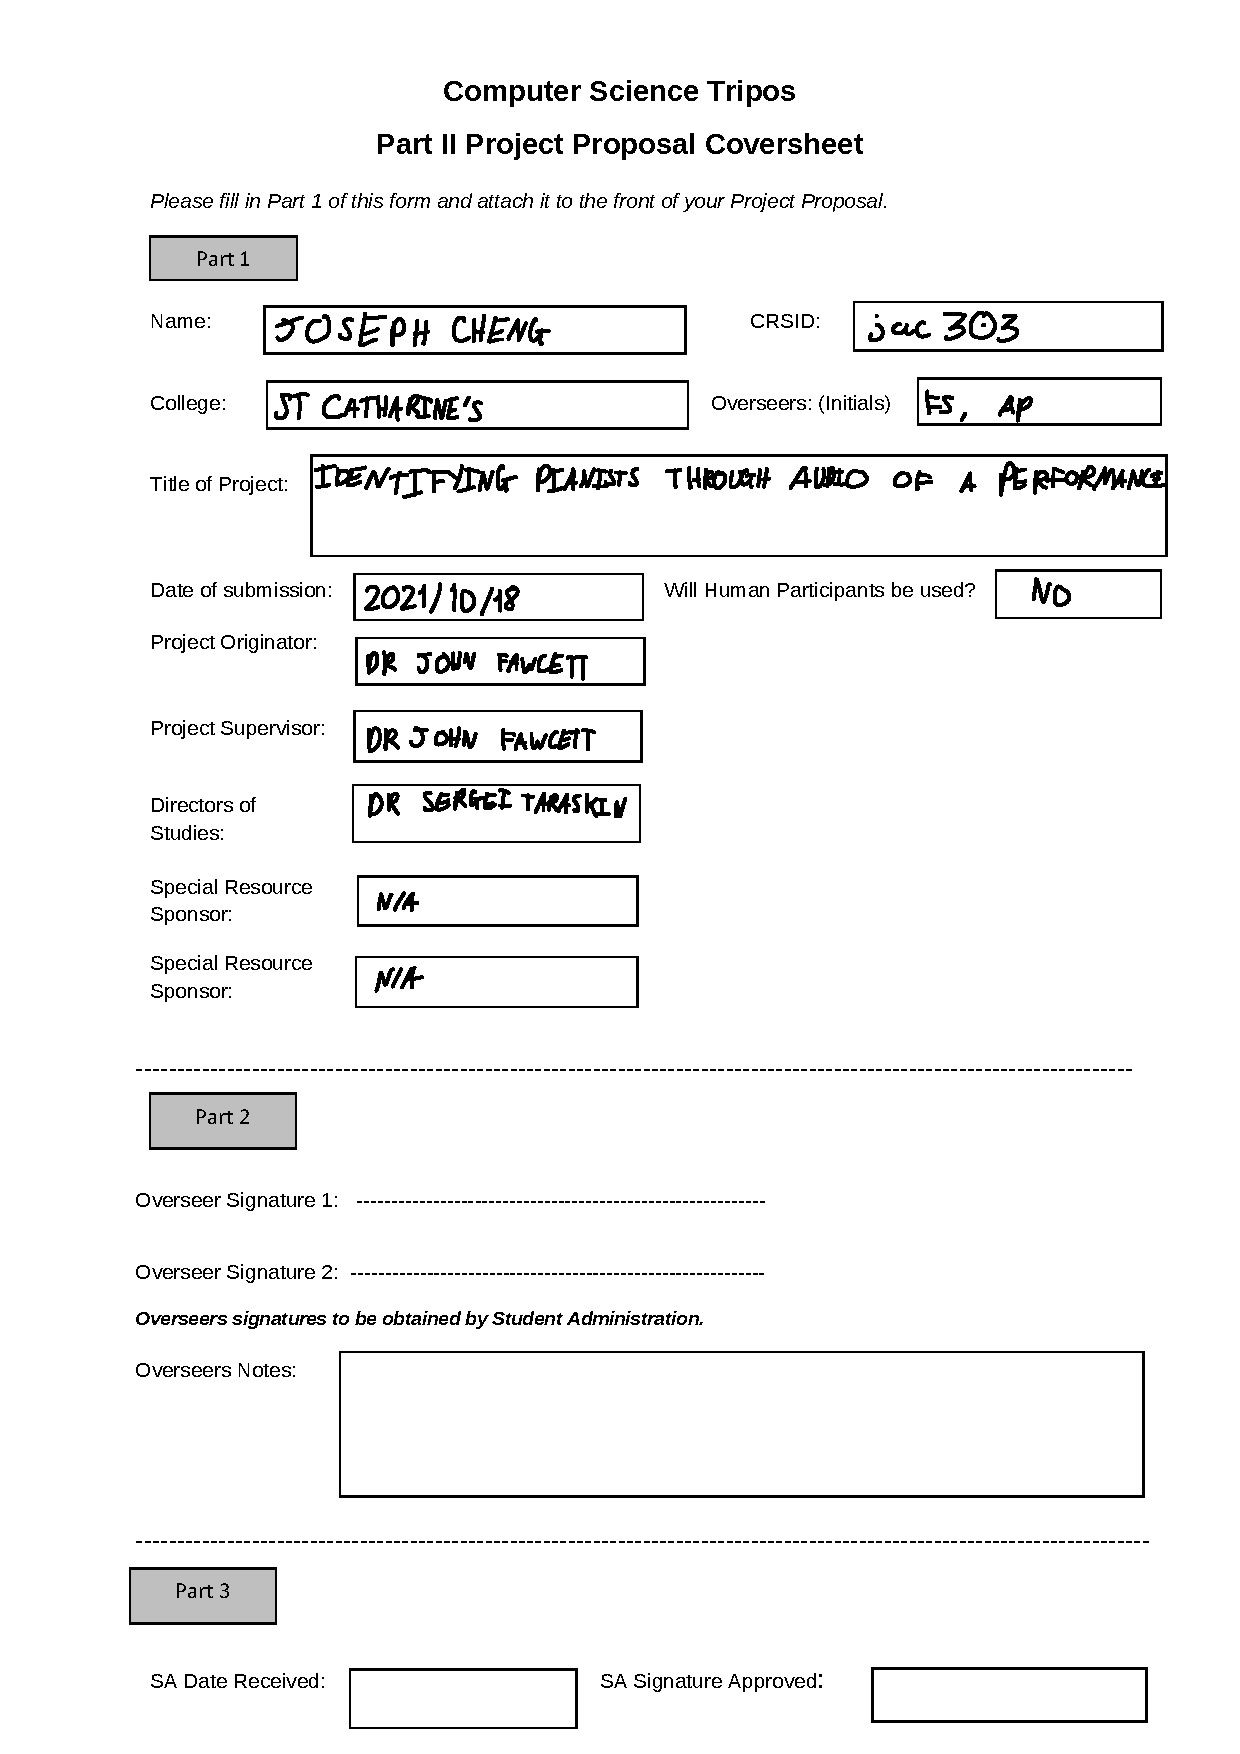
\includepdf[pages=-, pagecommand={}, width=\textwidth]{proposalform_filled.pdf}
\section{Introduction and Description of the Work}

Individuals will have many behavioural traits that could be unique enough to identify them. For example, work has been done to identify the author of a written document based on the handwriting of the author. Similarly to how handwriting can be used to identify an author, it is acknowledged that the performer of a piece of music might be able to be identified from a performance. This project aims to investigate the identification of a performer of a piece of music based on qualities of how they play the piece, and compare which of these qualities are most useful, and how identification using these qualities holds up under variation, such as detuning the instrument, or the addition of background noise.

There are numerous ways that such an identification mechanism could be created. For example, a signature could be created based on microsecond timings of when keys are pressed, or on the distribution of amplitudes of notes, or on the variation of tempo throughout the performance.

Each identification system will store metrics of performed pieces, and upon performance of the same piece by the same pianist, the system will attempt to identify the pianist. A number of identification systems will be created, with an identification system for each combination of metrics possible.

To make an identification decision on a particular performance, a system will calculate the metrics of the performance, calculate similarity of each metric to the corresponding metric of each stored performance, and choose the performance with the highest aggregate similarity.

To evaluate these systems, I will create pianist profiles that store information about how an artificial pianist might play a piece. This might include information like the probability distribution of their note offsets, relative to the expected note start time, or the distribution of key amplitudes they will play, etc. Using MusicXML scores from OpenScore, MIDI can be generated from a score and a pianist profile, which will then be synthesized into audio in the form of a WAV file. This can then be used to generate a number of statistics: false positive rate, false negative rate, precision, recall, and f-score, which each system will be evaluated on.

\section{Starting Point}

I do not have any experience in digital signal processing, although there is overlap with the Digital Signal Processing with Computer Music unit of assessment which I am undertaking.

I already have experience programming in Python, which is the language I plan to build the systems in, and I have not yet written any code that will contribute to this project. I do not have any experience using the \texttt{mingus}, \texttt{fluidsynth}, and \texttt{music21} Python libraries which I plan to use for data synthesis, and I have a small amount of experience using the \texttt{NumPy} and \texttt{SciPy} libraries from IB Data Science, which I plan to use for the digital signal processing parts of the project.

There is a small amount of research on this topic. One paper attempts to use 5 different performance qualities for identification \cite{bernays14}, but this research uses MIDI, whereas I intend my project to use audio. Some research has been done on using a sung musical password, taking into account the timbre of a singer’s voice \cite{prakash16}, but none on an instrument. There is, however, surrounding research that will be used, such as segmenting music into beats and estimating tempo \cite{ellis07}, or attempting to calculate the notes played in an audio signal \cite{li12}.

\section{Substance and Structure of the Project}

\subsection{Core Deliverables}

This project will consist of a number of different components:

\begin{itemize}
    

  \item Metric calculators: these will form the basis for construction of each musical identification system, and will calculate some metric about a performance that tries to capture some unique quality of a pianist’s playing. At a minimum, these metric calculators will be developed:

    \begin{itemize}
      \item Tempo variation over time: this metric intends to capture the interpretation of a piece by a pianist based on the average time between beats. This will use the techniques outlined by Ellis \cite{ellis07}.

      \item Dynamics over time: this metric intends to capture the interpretation of a piece by a pianist based on how the dynamics of the performance change over time.

      \item Chroma vector extraction: this metric intends to capture the tonal characteristics of the piece as it is played using the 12-tone system.

      \item Note offsets: this metric intends to capture timings of notes in the performance of the piece, as opposed to the expected timings based on the estimated tempo at a particular point.

      \item Timbre extraction: this metric intends to capture the timbre of the instrument.
    \end{itemize}

  \item Metric similarity: For each metric, I will implement a mechanism that is able to compare two metrics (i.e. from a stored performance, and from a performance we are trying to identify) and return a similarity score.

  \item Data synthesis: in order to test each identification system, I will need to develop a system which is able to generate data that can be used to evaluate the identification systems. This will involve creating pianist profiles, generating MIDI data from a score using each pianist profile, and synthesizing this MIDI data into audio. This will also involve the addition of variation to the signals such as by introducing background noise, which I intend to either synthesise (e.g. white noise), or obtain through \texttt{www.freesound.org}.

\end{itemize}

\subsection{Possible Extensions}
One extension would be to add metrics and perform additional evaluation for use with instruments other than pianos, which potentially could introduce qualities that the piano cannot create, such as pitch bends, or microtonal notes.

In order to create better pianist profiles, some work could be done in either generating pianist profiles from real pianist performances, or in attempting to work out what fingers each note will be played with, or which hand each note is played with to generate more ‘real’ MIDI data.

Another extension to this project would be to attempt this identification with real pianists, instead of artificial pianists, to see to what extent the musical identification techniques developed work on real pianists.

\section{Success Criteria}

The project will be successful if the following criteria are met:
\begin{itemize}
    
  \item
Each of the core deliverables is successfully implemented and it can be demonstrated that they work as intended

\item
A quantitative comparison is performed of each of the identification systems developed using the synthesized data
\end{itemize}

\section{Work Plan}

\begin{itemize}
    
  \item \textbf{Slot 1}: 2021/10/15 - 2021/10/28 \hspace*{\fill}Michaelmas Term Week 2-3

Read literature on digital signal processing, like Understanding Digital Signal Processing by R.G. Lyons. Investigate the use of the mentioned Python libraries. Read and understand research on tempo inference, and look into how the timbre of a sound can be quantitatively represented.

\textbf{Milestone}: Produce LaTeX source for a document explaining important DSP concepts, tempo inference, and timbre measurement that can be shown to my supervisor.

\item
  \textbf{Slot 2}: 2021/10/29 - 2021/11/11 \hspace*{\fill} Michaelmas Term Week 4-5

Complete implementation of data synthesis, such that a MusicXML score can be entered and piano audio can be synthesized, and implement pianist profiles such that audio can be generated from different ‘pianists’, and variation can be added to the signals.

\textbf{Milestone}: Audio from some MusicXML scores can be generated and shown to my supervisor, and furthermore the metric calculators from Slot 2 can be used on the generated audio.

\item
  \textbf{Slot 3}: 2021/11/12 - 2021/11/25 \hspace*{\fill}Michaelmas Term Week 6-7

Complete implementation of the metric calculators.

\textbf{Milestone}: Code for the metric calculators can be shown to my supervisor, and using the data synthesis system from slot 2, example metrics can be calculated from some test data.

\item
  \textbf{Slot 4}: 2021/11/26 - 2021/12/09 \hspace*{\fill}Michaelmas Term Week 8-Christmas Holiday Week 1

Write metric similarity calculators for each implemented metric.

\textbf{Milestone}: Test data can be generated using the data synthesis system and example metric similarity scores for each metric can be produced.

\item
  \textbf{Slot 5}: 2021/12/10 - 2021/12/23 \hspace*{\fill}Christmas Holiday Week 2-3

Slack period: Complete any milestones that were not delivered in their slot. Work on extensions if there are no such milestones.

\textbf{Milestone}: Every previous milestone deliverable can be shown to have been completed to my supervisor.

\item
  \textbf{Slot 6}: 2021/12/24 - 2022/01/06 \hspace*{\fill}Christmas Holiday Week 4-5

Write the progress report and the progress presentation. Work on extensions if there is time to do so. The deadlines for these are still TBC, but I thought it would be better to work

\textbf{Milestone}: The progress report and presentation will have been completed and shown to my supervisor.

\item

  \textbf{Slot 7}: 2022/01/07 - 2022/01/20 \hspace*{\fill}Christmas Holiday Week 6-7

Discuss evaluation methods with my supervisor, and decide on a plan. Write a first draft of the Introduction chapter of the dissertation

\textbf{Milestone}: An evaluation plan will be created and sent to my supervisor, and the first draft of the Introduction chapter of the dissertation will be sent to my supervisor.

\item

  \textbf{Slot 8}: 2022/01/21 - 2022/02/03 \hspace*{\fill} Lent Term Week 1-2

Evaluate each of the core deliverables, and write a first draft of the Preparation chapter of the dissertation, and begin work on a first draft of the Implementation chapter of the dissertation.

\textbf{Milestone}: Evaluations of the core deliverables will be completed. A first draft of the Preparation chapter will be written and shown to my supervisor.

\item
  \textbf{Slot 9}: 2022/02/04 - 2022/02/17 \hspace*{\fill}Lent Term Week 3-4

Slack period: Complete any milestones that were not delivered in their slot. Work on extensions if there are no such milestones.

\textbf{Milestone}: Every previous milestone deliverable can be shown to have been completed to my supervisor.

\item
  \textbf{Slot 10}: 2022/02/18 - 2022/03/03 \hspace*{\fill}Lent Term Week 5-6

Complete the first draft of the Implementation chapter of the dissertation, and write a first draft of the Evaluation chapter of the dissertation.

\textbf{Milestone}: The Implementation and Evaluation chapters of the dissertation will both have been completed and shown to my supervisor.

\item
  \textbf{Slot 11}: 2022/03/04 - 2022/03/17 \hspace*{\fill}Lent Term Week 7-8

Write the Conclusion chapter of the dissertation, and work on any extensions.

\textbf{Milestone}: The first draft of my dissertation will have been completed and shown to my supervisor. Code from any extensions may also be available as a milestone.

\item
  \textbf{Slot 12}: 2022/03/18 - 2022/03/31 \hspace*{\fill}Easter Holiday Week 1-2

Slack period: Complete any milestones that were not delivered in their slot. Work on evaluating extensions if there are no such milestones.

\textbf{Milestone}: Every previous milestone deliverable can be shown to have been completed to my supervisor.

\item
  \textbf{Slot 13}: 2022/04/01 - 2022/04/14 \hspace*{\fill}Easter Holiday Week 3-4

Write a new revision of the dissertation based on feedback from my supervisor.

\textbf{Milestone}: A second draft of the dissertation will be completed and shown to my supervisor.

\item
  \textbf{Slot 14}: 2022/04/15 - 2022/04/28 \hspace*{\fill}Easter Holiday Week 5-6

Refine the dissertation even further using new feedback from my supervisor

\textbf{Milestone}: The final draft of the dissertation will have been completed.

\item
  \textbf{Slot 15}: 2022/04/29 - 2022/05/13 \hspace*{\fill}Easter Term Week 1-2

Make final changes and refinements to the dissertation, and finish any milestones not yet completed.

\textbf{Milestone}: Dissertation and code will be submitted.
\end{itemize}

\section{Resource Declaration}

Personal machine: I will be using my PC (AMD Ryzen 5 3600, 16GB RAM, 1TB hard drive and 512GB SSD) to develop the project. If a failure occurs with this computer, I have a backup laptop to continue development (Thinkpad X250 i5-5300U, 8GB RAM, 256GB SSD), and also have the finances to purchase another laptop at short notice in the case that this fails also. To prevent data loss, I will be using Git for version control and will backup weekly to a remote repository using GitHub.

\printbibliography



\end{document}
